%%%%%%%%%%%%%%%%%%%%%%%%%%%%%%%%%%%%%%%%%
% Beamer Presentation
% LaTeX Template
% Version 1.0 (10/11/12)
%
% This template has been downloaded from:
% http://www.LaTeXTemplates.com
%
% License:
% CC BY-NC-SA 3.0 (http://creativecommons.org/licenses/by-nc-sa/3.0/)
%
% Modified by Jeremie Gillet in November 2015 to make an OIST Skill Pill template
%
%%%%%%%%%%%%%%%%%%%%%%%%%%%%%%%%%%%%%%%%%

%----------------------------------------------------------------------------------------
%	PACKAGES AND THEMES
%----------------------------------------------------------------------------------------

\documentclass{beamer}

\mode<presentation> {

\usetheme{Madrid}

\definecolor{OISTcolor}{rgb}{0.65,0.16,0.16}
\usecolortheme[named=OISTcolor]{structure}

%\setbeamertemplate{footline} % To remove the footer line in all slides uncomment this line
%\setbeamertemplate{footline}[page number] % To replace the footer line in all slides with a simple slide count uncomment this line

\setbeamertemplate{navigation symbols}{} % To remove the navigation symbols from the bottom of all slides uncomment this line
}

\usepackage{graphicx} % Allows including images
\usepackage{booktabs} % Allows the use of \toprule, \midrule and \bottomrule in tables
\usepackage{textpos} % Use for positioning the Skill Pill logo
\usepackage{transparent} % For transparency with images
\usepackage{textcomp} % To print otherwise protected symbols e.g. <,>

\usepackage{ulem} % For strikethrough.

% For code displays
\usepackage{listings}
\usepackage{color}
\usepackage{amsmath}

% Allows side-by-side presentation notes
\usepackage{pgfpages}
\setbeameroption{show notes on second screen}

\definecolor{dkgreen}{rgb}{0,0.6,0}
\definecolor{gray}{rgb}{0.5,0.5,0.5}
\definecolor{mauve}{rgb}{0.58,0,0.82}

\lstset{frame=tb,
  language=python,
  aboveskip=3mm,
  belowskip=3mm,
  showstringspaces=false,
  columns=flexible,
  basicstyle={\small\ttfamily},
  numbers=none,
  numberstyle=\tiny\color{gray},
  keywordstyle=\color{blue},
  commentstyle=\color{dkgreen},
  stringstyle=\color{mauve},
  breaklines=true,
  breakatwhitespace=true,
  tabsize=3
}



%----------------------------------------------------------------------------------------
%	TITLE PAGE
%----------------------------------------------------------------------------------------

\title{Introduction to Git and Version Control} % The short title appears at the bottom of every slide, the full title is only on the title page
\subtitle{Lecture 1: Git ready!}

%\author{\textbf{James Schloss}} % Your name
\author{\textbf{Christopher Buckley}} % Your name
\institute[OIST] % Your institution as it will appear on the bottom of every slide, may be shorthand to save space
{
Okinawa Institute of Science and Technology \\ % Your institution for the title page
%\textit{james.schloss@oist.jp} % Your email address
}
\date{August 16, 2021} % Date of the presentation

\begin{document}

\setbeamertemplate{background}{\transparent{0.65}\includegraphics[width=\paperwidth]{SPbackground.png}} % Adding the background logo

\begin{frame}
\vspace*{1.4cm}
\titlepage % Print the title page as the first slide
\hfill \textbf{Original Slides by James Schloss, 2016}
\end{frame}

\setbeamertemplate{background}{} % No background logo after title frame

\addtobeamertemplate{frametitle}{}{% Adding the logo on the title screen after title frame
\begin{textblock*}{100mm}(.8\textwidth,-1.25cm)
\includegraphics[height=2cm]{SPwhite.png}
\end{textblock*}}


\begin{frame}
\frametitle{Overview} % Table of contents slide, comment this block out to remove it
\hfill
\parbox[t]{0.9\textwidth} {
\begin{minipage}[c][0.65\textheight]{\textwidth}
\tableofcontents % Throughout your presentation, if you choose to use \section{} and \subsection{} commands, these will automatically be printed on this slide as an overview of your presentation
\end{minipage}
}
\end{frame}
\note{
	\begin{itemize}
	\item Git is different from github
	\item Why Git? I'll tell you what my motivations are, but what are your motivations for being here? 
	\end{itemize}
}

%----------------------------------------------------------------------------------------
%	PRESENTATION SLIDES
%----------------------------------------------------------------------------------------

%------------------------------------------------

\section{Why Git?}

\begin{frame}
\frametitle{Why Git?}
\begin{itemize}
\item Version control
\item Easily compare and merge changes between any version
\item Organize your work items
\end{itemize}
\begin{center}\includegraphics[width=0.9\textwidth]{beforeafter.jpg}\end{center}
\end{frame}
\note{
	Imagine I asked you to remove the red sharpie marker from the left hand side?
	\begin{itemize}
	\item Difficulty finding it
	\item Could dive right in, but might get poked by lot of sharp things on the way in
	\item Or you could dump everything out and start all over
	\end{itemize} 
}

\begin{frame}
\frametitle{Why Git?}
\begin{center}\includegraphics[width=0.5\textwidth]{stackedChairs.jpeg}\end{center}
\end{frame}
\note{
	Imagine I asked you to remove this chair. What difficulties would you face?
	\begin{itemize}
	\item How to access it safely
	\item Can't remove it without fearing everything will fall
	\end{itemize} 
}

\subsection{Traditional vs. Git Versioning}

\begin{frame}[fragile]
\frametitle{Traditional vs. Git Versioning}
\begin{itemize}
\item What changed when
\item Not limited to file name length to inform user of changes
\end{itemize}
\begin{center}\includegraphics[width=0.9\textwidth]{versioning.png}\end{center}
\note{This is just a VERY limited toy example, but to just want to show how I versioned in my master's thesis compared to now using git. We'll get to the actual useful stuff later. }
\end{frame}

\section{What is Git}

\subsection{Three Main Parts (Working Directory, Stage, Repository)}

\begin{frame}[fragile]
\frametitle{What is git?}
\begin{itemize}
\item A \textbf{Working Directory}: Just a folder where your files are
\item A \textbf{Staging Area}: A place to organize what exactly you want to version and what you don't
\item A \textbf{Repository}: Where the magic happens. 
\end{itemize}
\includegraphics[width=\textwidth]{git3MainItems.png}
\end{frame}
\note{
This chart might not make much sense now, but I hope it will before the end of these slides

Whether you realize it or not, you are already familiar with the "Working Directory". I'll save the staging area for a bit later, but first lets talk about what a repo is.}

\begin{frame}[fragile]
\frametitle{Repositories}
\begin{itemize}
\item A \textbf{repository} is a container for both your project data and all the items that allow interactions with git commands.
\begin{itemize}
\item There are many sites to host your repository on (github, bitbucket), including your own local machine.
\item All of the essential parts of your repository can be found in the \textbf{.git} directory
\item GitHub (a website hosting Git repositories) $\neq$ Git (a set of tools for creating and managing those repositories).
\end{itemize}
\end{itemize}
\includegraphics[width=\textwidth]{Storage.jpg}
\end{frame}

\section{How to Use Git}

\subsection{The Terminal}

\begin{frame}[fragile]
\frametitle{Terminal Talk}
\begin{columns}
\column{0.7\textwidth}
\begin{itemize}
\item There are multiple GUIs available for Git, such as one from GitHub called the \textbf{GitHub Desktop}. We will not be using this for \sout{religious} perfectly scientific reasons.
\item These reasons primarily revolve around flexibility and improved understanding of the Git tools.
\item Everything we do will be usable on Deigo.
\item The \textbf{Pro Git} book is available online at \href{https://git-scm.com/book/}{\textbf{\color{blue}{git-scm.com/book}}}
\item There is a cheatsheet for Git available here: \href{https://www.git-tower.com/learn/cheat-sheets/git}{\textbf{\color{blue}{https://www.git-tower.com/learn/cheat-sheets/git}}}
\end{itemize}
\column{0.3\textwidth}
\includegraphics[width=\textwidth]{terminal.png}
\end{columns}
\end{frame}
\note{
	\begin{itemize}
	\item I personally struggled with the terminal interface at first because most of the man pages use so much vocab I don't know to explain terms I don't know. Hopefully by the end of this mini-course you'll have the basic vocab down so you 	can help yourselves more efficiently going forward.
	\end{itemize}
}

\subsection{Create a repo}

\begin{frame}[fragile]
\frametitle{Create a Repo(sitory)}
\begin{columns}
\column{0.7\textwidth}
Let's \textbf{git} started.
\begin{itemize}
\item To initialize a git repository, simply type \textbf{git init} in a directory (preferably empty for now)
\item This creates a folder \textbf{.git/}, where all your repository information is held.
\end{itemize}
\column{0.3\textwidth}
\includegraphics[width=\textwidth]{git.jpg}
\end{columns}
\end{frame}

\begin{frame}[fragile]
\frametitle{Create an Empty Repo}
    \begin{block}{EXERCISE}
        \begin{enumerate}
        \item Open a terminal
        \item Create a new directory called \textbf{myFirstRepo} and enter it.
	 \item This is your Working Directory. Thats it!
	 \item Run \textbf{git init} in your Working Directory.
        \item Take a peak in the newly created .git directory but don't touch anything quite yet.
        \end{enumerate}
    \end{block}

\end{frame}

\subsection{Commits}

\begin{frame}[fragile]
\frametitle{Commits}
\begin{itemize}
\item Conceptually similar to "versions"
\item The more effort you put into crafting these the more helpful they are in the future.
\end{itemize}
\includegraphics[width=0.9\textwidth]{git_commit.png}
\end{frame}
\note{
	\begin{itemize}
	\item Using git in and of itself does not mean you will have better versioning. 
	\item We need to make GOOD commits for git to have any significant benefit.
	\item By "versions" I mean what you may be used to seeing in dropbox or similar backup schemes.
	\item Git at its worst acts quite similar to this, but if used properly can add so much more.
	\item To clarify with a more visual example, I made a house using legos. (Lego photos on next slides). 
	\end{itemize} 
}

\begin{frame}[fragile]
	\frametitle{Commits}
	\begin{figure}
		\centering
		\includegraphics[width=0.5\textwidth]{./legoCommits/badCommits/1added_some_stuff.jpg}
	\end{figure}
	\note{Added some stuff}
\end{frame}

\begin{frame}[fragile]
	\frametitle{Commits}
	\begin{figure}
		\centering
		\includegraphics[width=0.5\textwidth]{./legoCommits/badCommits/2added_more_stuff.jpg}
	\end{figure}
	\note{Added some more stuff}
\end{frame}

\begin{frame}[fragile]
	\frametitle{Commits}
	\begin{figure}
		\centering
		\includegraphics[width=0.5\textwidth]{./legoCommits/badCommits/5added_roof_Housev1.0.jpg}
	\end{figure}
	\note{Done! Now lets say we found an error in the western wall. Which commit was that added in?}
\end{frame}

\begin{frame}[fragile]
	\frametitle{Commits}
	\begin{figure}
		\centering
		\includegraphics[width=0.5\textwidth]{./legoCommits/goodCommits/1set_foundation.jpg}
	\end{figure}
	\note{Added the foundation}
\end{frame}

\begin{frame}[fragile]
	\frametitle{Commits}
	\begin{figure}
		\centering
		\includegraphics[width=0.5\textwidth]{./legoCommits/goodCommits/2added_walls.jpg}
	\end{figure}
	\note{Added the walls}
\end{frame}

\begin{frame}[fragile]
	\frametitle{Commits}
	\begin{figure}
		\centering
		\includegraphics[width=0.5\textwidth]{./legoCommits/goodCommits/3added_window.jpg}
	\end{figure}
	\note{Added the window}
\end{frame}

\begin{frame}[fragile]
	\frametitle{Commits}
	\begin{figure}
		\centering
		\includegraphics[width=0.5\textwidth]{./legoCommits/goodCommits/4added_door.jpg}
	\end{figure}
	\note{Added the door}
\end{frame}

\begin{frame}[fragile]
	\frametitle{Commits}
	\begin{figure}
		\centering
		\includegraphics[width=0.5\textwidth]{./legoCommits/goodCommits/5added_roof_Housev1.0.jpg}
	\end{figure}
	\note{Added the roof}
\end{frame}

\subsection{The Stage (Staging Area, or Index)}

\begin{frame}
\frametitle{Staging Changes}
\begin{center}
\includegraphics[width=0.75\textwidth]{lifecycle.png}
\end{center}
\begin{itemize}
\item A new file is initially \textbf{untracked}
\item When you use \textbf{git add}, it moves to the staging area and becomes \textbf{staged}
\item After being committed (using \textbf{git commit}), a file is up-to-date and considered \textbf{unmodified}
\item Changing a file makes it modified, but doesn't add it to the staging area
\end{itemize}
\end{frame}
\note{So how do we construct or make these GOOD commits? By using the Staging Area or Index. Next we'll discuss what this is and how to use it to make GOOD commits.}

\begin{frame}[fragile]
\frametitle{Currating the Stage before Committing}
\begin{columns}
\column{0.7\textwidth}
\begin{itemize}
\item Check what is on the stage with \textbf{git status}. Anything in \textcolor{dkgreen}{green} is staged.
\item If you wish to unstage all changes, simply type \textbf{git reset}. This will remove everything from the stage, but keep your working directory untouched. 
\item \textbf{git reset} will work for individual files as well
        \begin{lstlisting}
git reset <file>
        \end{lstlisting}
\end{itemize}
\column{0.3\textwidth}
\includegraphics[width=\textwidth]{the-hook.jpg}
\end{columns}
\end{frame}
\note{
	\begin{itemize}
		\item As you saw a few slides ago. Adding messy or unnecessary commits doesn't help anyone. Lets discuss how to make meaningful helpful commits using the stage. There are various ways to fix bad commits, but it takes a whole lot less work to do it right the first time.
		\item Git works best with the workflow Prof. Doya often and rightly reminds of; start with something simple and work our way up.
	\end{itemize}
}
\begin{frame}[fragile]
\frametitle{Try out the Stage}
	\begin{block}{EXERCISE}
		\begin{enumerate}
		\item Create a new emtpy file \textbf{myfile.txt}
		\item Check the status of everything with \textbf{git status}
		\item Add \textbf{myfile.txt} to the stage vis \textbf{git add myfile.txt}
		\item Check the status of everything again with \textbf{git status}. What changed?
		\item Unstage the changes with \textbf{git reset myfile.txt}
		\item Check the status of everything again with \textbf{git status}. What changed?
		\end{enumerate}
	\end{block}

\end{frame}


\begin{frame}[fragile]
\frametitle{Committing from the Stage}
\begin{itemize}
\item Git keeps track of \textbf{commits}. Check these commits with \textbf{git log}. There's plenty of options to show only what you want or everything under the sun. 
\item \textbf{git status} checks any changes since the last commit.
\item \textbf{git commit} commits everything in the \textit{staging area} - git status shows these files in {\color{dkgreen}green} by default.
\end{itemize}
\end{frame}

\subsection{Making Commits}

\begin{frame}[fragile]
\frametitle{Making Commits}
    \begin{block}{EXERCISE}
        \begin{enumerate}
        \item Repoen your \textbf{myFirstRepo} from before
	 \item Add the \textbf{myFile.txt} back to the stage with \textbf{git add myFile.txt}
	 \item Check the status of the stage with \textbf{git status}
        \item Once satisfied with what is in the stage and you're ready to commit, go ahead and do so with \textbf{git commit} to add your new file to the git repository. Be sure to add a meaningful commit message!
        \item Check the \textbf{git log}.
	 \item Check the \textbf{git status}
 	 \item Add a line of text to \textbf{myFile.txt} and save it.
	 \item Check the status of the stage with \textbf{git status}
	 \item Check the differences in the file with \textbf{git diff}
	 \item Once satisfied with your changes, add it back to the stage and commit. 
        \end{enumerate}
    \end{block}
\end{frame}

\subsection{Checking Out Past Commits}

\begin{frame}[fragile]
\frametitle{Checking out your past commits}
\begin{itemize}
\item \textbf{git checkout} allows you to view the repository at any commit (found with \textbf{git log}).
\item You may also checkout specific files like so: 
        \begin{lstlisting}
git checkout a1e8fb5 hello.py
        \end{lstlisting}
\item Note that the most recent commit is \textbf{HEAD} and the one just before that is \textbf{HEAD$\mathbf{\sim}$1}
\begin{center}\includegraphics[width=0.7\textwidth]{head.png}\end{center}
\end{itemize}
\end{frame}

\begin{frame}[fragile]
\frametitle{Checkout Your History}
    \begin{block}{EXERCISE}
        \begin{enumerate}
	 \item Add a second line of text to \textbf{myFile.txt} and save it.
	 \item Add these changes to the stage with \textbf{git add myFile.txt} and check the status with \textbf{git status}
        \item Once satisfied with what is in the stage and you're ready to commit, use \textbf{git commit} to add your new file to the git repository.
        \item Check the \textbf{git log}. You should have three commits by now.
	 \item Go checkout each of the commits with \textbf{git checkout \textlangle{}HASH\textrangle{}}, \textbf{git checkout HEAD\textasciitilde1}, or \textbf{git checkout HEAD\textasciitilde2}
	 \item See whats different with \textbf{ls -al} or \textbf{git status} or just open \textbf{myfile.txt} in your favorite text editor
	 \item When you are satisfied that your commit history is as expected you can return to the most recent commit with \textbf{git checkout master} (Note this could be \textbf{git checkout main} depending on your version of git.)
        \end{enumerate}
    \end{block}
\end{frame}

\begin{frame}[fragile]
\frametitle{Git Generally Only Adds}

\begin{itemize}
\item After you commit something it is fairly difficult to remove it.
\item This is a double edged sword. Low risk of losing anything permanently. High risk of creating a HUGE repo. 
\item Keep your repository clean! Do your best to commit as few images and data files as possible!
\item You can do this by ignoring certain file extensions in a \textbf{.gitignore} file.
\item Great templates for projects of many types found at \textbf{\href{https://github.com/github/}{https://github.com/github/gitignore}}
\end{itemize}
\begin{columns}
\column{0.5\textwidth}
\begin{lstlisting}
# Example gitignore configuration
*.log
*.tar
*.gz
*.exe
*.dat
*.lvlps
\end{lstlisting}
\column{0.5\textwidth}
\includegraphics[width=\textwidth]{IIB.jpg}
\end{columns}
\end{frame}
\note{My robot repo is now 500GB due to huge Solidworks CAD files.}

\begin{frame}[fragile]
\frametitle{Quick Exercise}
    \begin{block}{EXERCISE}
        \begin{enumerate}
        \item Touch multiple files with various extensions, one of which should be \textbf{.dat}.
        \item Ignore the \textbf{.dat} file, but commit all the others.
        \item Be sure to write a clear message describing what you did.
        \item Check the \textbf{git log}
        \end{enumerate}
    \end{block}

\end{frame}

\begin{frame}
	\frametitle{Modifying Previous Commits}
	\begin{itemize}
		\item If you commit something that turns out to be a mistake, don't worry! There are plenty of tools to rework commits.
		\item Some are more powerful (and potentially distructive than others)
		\item Non-destructive: (Leaves history intact)
		\begin{itemize}
			\item \textbf{revert}
		\end{itemize}
		\item Potentially destructive: (Changes history)
		\begin{itemize}
			\item \textbf{reset}
			\item \textbf{rebase}
		\end{itemize}
		\item Danger Zone: (Can erase history)
		\begin{itemize}
			\item \textbf{reflog}
		\end{itemize}
		\item Note: These tools may take some time to conceptualize, so I encourage you to play around with them in your toy environments (e.g. myFirstRepo) a fair bit before trying them out on your actual code base. 
	\end{itemize}
\end{frame}

\subsection{Revert}

\begin{frame}[fragile]
	\frametitle{Using Revert}
	\begin{itemize}
		\item \textbf{git revert \textlangle{}HASH\textrangle{}} makes a new commit showing what you reverted.
		\item Pro: This is very useful for public repos where you want to show exactly what you've undone to others.
		\item Con: Can make your commit history messy if used too often. 
	\end{itemize}
\end{frame}

\begin{frame}[fragile]
	\frametitle{Using Revert}
	\begin{block}{EXERCISE}
		\begin{enumerate}
			\item Make a few commits to your \textbf{myFirstRepo} if you don't have any already. Make sure they are simple for now (just single line additions). Use \textbf{git log} to understand your current git history and \textbf{cat myfile.txt} to understand the contents of your file before reverting.
			\item Find a commit you want to revert using \textbf{git log} and \textbf{git show} or \textbf{git diff}. Ensure the commit you choose is just the addition of a single line. 
			\item Revert that commit with \textbf{git revert \textlangle{}HASH\textrangle{}} or \textbf{git revert HEAD\textasciitilde\textlangle{}\#\textrangle{}} Use \textbf{git log} to understand your current git history. Use \textbf{cat myfile.txt} to again understand the contents of your file after reverting.
		\end{enumerate}
	\end{block}
\end{frame}

\subsection{Reset}

\begin{frame}[fragile]
	\frametitle{Using Reset}
	\begin{itemize}
		\item You may remember the \textbf{git reset} command to remove things from the Staging Area (undoing staging)
		\item We can also use \textbf{git reset} to undo commits. 
		\item This is a great way to undo fairly recent commits (one or two before), but not the ideal tool for doing anything further than that. 
		\item When you use \textbf{git reset HEAD\textasciitilde1} you undo your most recent commit but retain all the changes the commit made. This is useful if you accidentally included a file in a commit and want to go back, and remake the commit.  
	\end{itemize}
\end{frame}

\begin{frame}[fragile]
	\frametitle{Using Reset}
	\begin{block}{EXERCISE}
		\begin{enumerate}
			\item Make a new commit with a single line addition to myfile.txt and add a new file called "BIGBINARY". 
			\item Make sure you have a clean working directory (no local changes compared to most recent commit) with \textbf{git status}
			\item Use \textbf{git show} to show the changes made by your most recent commit. Hopefully this should show the single line addition to myfile.txt and the newly added BIGBINARY file.
			\item Use \textbf{git reset HEAD\textasciitilde1} to undo this commit but keep the single line addition and BIGBINARY in the working directory (Your work is not undone, just the commit).
			\item Use \textbf{git status} to see that this line addition is still in your text file, but \textbf{git log} no longer shows the commit
			\item Make a new GOOD commit by adding only myfile.txt to the stage and not BIGBINARY.
		\end{enumerate}
	\end{block}
\end{frame}

\subsection{Rebase}

\begin{frame}[fragile]
	\frametitle{Using Rebase}
	\begin{itemize}
		\item \textbf{git rebase} rewrites the commit history by starting from specified base commit and choosing what to do with each commit all the way to the current HEAD.
		\item Pro: Great for removing WIP commits or otherwise meaningless commits. Use it to clean up your local history before pushing to a public repo.
		\item Con: This has the possiblity to create a lot of conflicts if used in a shared repo (as one person's history will differ from another). Generally rebase should not be used to modify any commits you have pushed to a public repo. 
		\item Generally I recommend using \textbf{git rebase -i} for beginners as this shows you what is going on each step of the way.
	\end{itemize}
\end{frame}

\begin{frame}[fragile]
	\frametitle{Using Rebase}
	\begin{block}{EXERCISE}
		\begin{enumerate}
			\item Make sure you have at least 5 commits to your \textbf{myFirstRepo}.
			\item Making at least one of these a meaningless WIP commit. 
			\item Use \textbf{git log} to find the earliest commit that was bad (first WIP commit). Copy the HASH from the commit \textbf{just prior} to this WIP commit. We want to rebase our current HEAD not on the WIP commit, but just before it so we can remove or fix the WIP commit. 
			\item Use \textbf{git rebase -i \textlangle{}HASH\textrangle{}} and follow the instructions
		\end{enumerate}
	\end{block}
\end{frame}

\begin{frame}[fragile]
\frametitle{Branches}
\begin{itemize}
	\item Separating workflows
	\item Using them does not imply you are working with others. 
	\item You can make/delete them anytime, but the goal is to develop something that works, then merge it into your main/master branch.
\begin{center}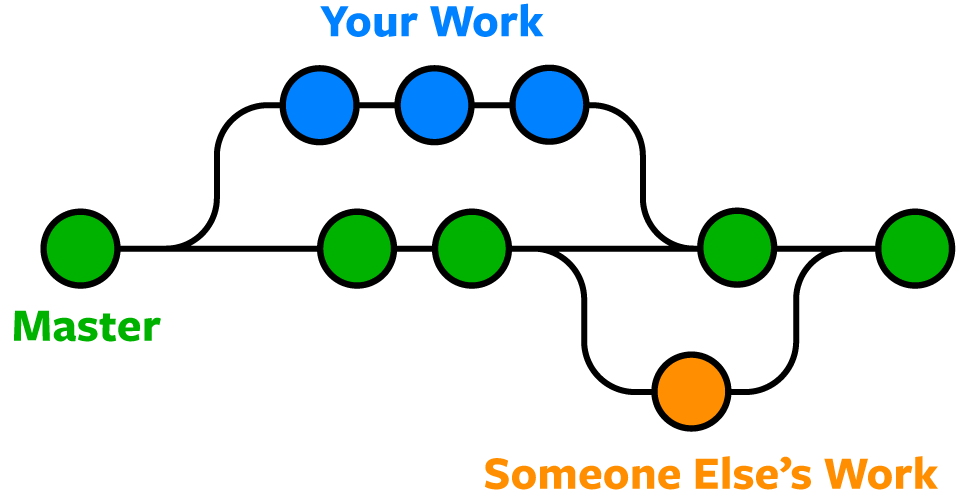
\includegraphics[width=0.7\textwidth]{branch.png}\end{center}
\end{itemize}
\end{frame}
\note{
	\begin{itemize}
		\item When you want to develop something separately (New features, refactoring, hacking away) but don't want to affect your main workflow.
		\item Make a new branch before doing something you think will break the code, or do something you think will be nontrivial (more than one commit). 
		\item With the house example, think separation of the development of garage or porch. Or think about remodeling the interior while someone else works on the exterior.  
	\end{itemize}
}

\begin{frame}[fragile]
\frametitle{Branches: Creating and Deleting Them}
	\begin{block}{EXERCISE}
	\begin{enumerate}
		\item \textbf{git branch my2ndBranch } Create a new branch at HEAD
		\item \textbf{git checkout my2ndBranch} to check it out
		\item Make 2 WIP commits (empty files, single line additions, etc).
		\item \textbf{git log --all} or \textbf{git log --pretty='format:\%C(auto)\%h \%d \%s, \%C(green)\%ad)' --all --graph --abbrev-commit --notes --date=relative} for a prettier log/tree.
		\item \textbf{git branch -d my2ndBranch}: Delete a branch (Git warns you)
		\item \textbf{git checkout master}: Checkout master branch before deleting.
		\item \textbf{git branch -d my2ndBranch}: Delete a branch (Git warns you)
		\item \textbf{git branch -D my2ndBranch}: Delete a branch
		\item Shortcut: \textbf{git checkout -b my2ndBranch}: Create a new branch @ HEAD and then check it out.
	\end{enumerate}
\end{block}
\end{frame}
\note{Lets take a look at how to create, delete and play around with branches}

\section{Working Online}

\begin{frame}
\frametitle{\textbf{git} with it!}
\begin{columns}
\column{0.7\textwidth}
Now we move to the fun* stuff: working with \textbf{online repositories}.
\begin{itemize}
\item For this, we will be using \textbf{github}.
\item We'll begin by creating a GitHub repository using the \href{www.github.com}{website}.
\begin{itemize}
\item If we're working on a project that's already hosted on a remote Git server, we can skip this step.
\end{itemize}
\item Next, we use \textbf{git clone} to download a copy.
\item From here, you can do the following:
\begin{itemize}
\item \textbf{git push} to push any changes you may have to the online repository.
\item \textbf{git pull} to take any changes from the repository.
\end{itemize}
\end{itemize}
\column{0.28\textwidth}
\includegraphics[width=\textwidth]{clone.jpg}
\end{columns}

*Here, the word \textit{fun} is subject to interpretation.
\end{frame}
\note{It may be better (especially for beginners) to use git fetch or git remote update rather than pull}

\begin{frame}[fragile]
\frametitle{Quick Exercise}
    \begin{block}{EXERCISE}
        \begin{enumerate}
        \item Fork the \textbf{\href{https://github.com/oist/skillpill-git}{https://github.com/oist/skillpill-git}} repository using a browser.
        \item Clone the forked repository* to your local disk:
        \begin{lstlisting}
git clone git@github.com:<git_user_name>/skillpill-git.git
        \end{lstlisting}
        or
        \begin{lstlisting}
git clone https://github.com/<git_user_name>/skillpill-git.git
        \end{lstlisting}
        \item Make some simple commits and test the process of \textbf{push}ing and \textbf{pull}ing stuff from that repo.
        \end{enumerate}
    \end{block}

*The examples here show cloning the SkillPill Git repository - replace the links as appropriate!
\end{frame}

\section{Wrap Up}

\begin{frame}
\frametitle{What it will feel like...}
\begin{columns}
\column{0.6\textwidth}
\begin{itemize}
\item git is not intuitive to start with, but it's %the best way to work collaboratively with other people.
a powerful tool for storing and restoring history, and working collaboratively with other people.
\item The more you use it, the more you will like it. Think Stockholm syndrome.
\item Operations that you use frequently will become easy.
\item Operations you use infrequently, you can Google!
\end{itemize}
\column{0.4\textwidth}
\includegraphics[width=\textwidth]{gitxkcd.png}
\end{columns}
\end{frame}

\begin{frame}
\frametitle{Final Comments}
\begin{columns}
\column{0.7\textwidth}
\begin{itemize}
\item git is weird. It's not intuitive, but it's the best way to collaborate with people on open projects.
\item It's also great even if you don't collaborate!
\item Whenever you are using git, think about other people and how they will perceive your comments. \textbf{Would you be able to understand your own cryptic commit messages?}
\item You will make mistakes. Don't worry about it. Your entire history is backed up already. Learn from your mistakes and don't make them again!
\item Read error messages carefully - they can be useful/informative/instructive.
\end{itemize}
\column{0.3\textwidth}
\includegraphics[width=\textwidth]{light-bulb.jpg}
\end{columns}
\end{frame}

\end{document} 

